% beamer for weekly report
% Created by Zihan on 2023-06-14

% turn off sans-serif math
\documentclass[11pt]{beamer}

% Packages
% \Sum
\usepackage{amsmath}
% \coloneqq
\usepackage{mathtools}
% bookmark
\usepackage{bookmark}

% theme
\usetheme{default}
\usefonttheme{serif}

% title
\title{Weekly Report}

% author
\author{Zihan}

% date
\date{\today}

% Document
\begin{document}

% first page
% tell the supervisor that what I think of n-gram
\begin{frame}
    \frametitle{N-gram}

    $n$-gram is a choice to represent the word, the sentence, or the document. It is originally used to predict the next word in a sentence.

    \begin{block}{Example for Bi-gram}
        $w_1$ \fbox{$w_2$ $w_3$} $w_4$

        where the ``$w_2$ $w_3$'' is the bi-gram.
    \end{block}

    To calculate the probability of ``$b_n$'' ($b_i = w_iw_{i+1}$), using Markov assumption, we have
    \begin{align*}
        P\left(b_{1: n}\right) & =P\left(b_1\right) P\left(b_2 \mid b_1\right) P\left(b_3 \mid b_{1: 2}\right) \ldots P\left(b_n \mid b_{1: n-1}\right) \\
                               & =\prod_{k=1}^n P\left(b_k \mid b_{1: k-1}\right)
    \end{align*}

\end{frame}

% second page
% My thought of n-gram and co-clustering

% it uses Markov assumption and gets the 共现概率 for each two words, and then we may get the 共现概率 matrix which is similar to the compatibility matrix in co-clustering. 

\begin{frame}
    \frametitle{N-gram and Co-clustering: A Conceptual Link}
    \begin{block}{From N-gram to Co-clustering}
        \begin{itemize}
            \item Markov Assumption: This principle is used to calculate the co-occurrence probability for each pair of words.
            \item Co-occurrence Probability Matrix: The calculated probabilities form a matrix, which is conceptually similar to the compatibility matrix used in co-clustering.
        \end{itemize}
    \end{block}
    \begin{block}{Co-occurrence Probability Matrix}
        \begin{equation*}
            p_{i j} \coloneqq P\left(b_i \mid b_j\right) = P\left(b_i | b_{i-1}\right) P\left(b_{i-1} | b_{i-2}\right) \ldots P\left(b_{j+1} | b_j\right)
        \end{equation*}
    \end{block}
\end{frame}    






% I want to solve the problem of LLM: model too big, and the training process is too slow

\begin{frame}
    \frametitle{Challenges in Training Large Language Models}
    \begin{columns}[T,onlytextwidth]
        \column{0.6\textwidth}
        \begin{block}{Training Duration is very Long}
            \begin{itemize}
                \item Model Size: Larger models require more resources and time.
                \item Dataset Size: Ensemble Learning, parallel computing, via partitioning the dataset, is a common solution.
            \end{itemize}
        \end{block}
    
        \begin{block}{Partitioning Problem}
            \begin{itemize}
                \item Random Partitioning: A common but problematic method due to it divides the related data into different parts.
            \end{itemize}
        \end{block}

        \column{0.3\textwidth}
        \begin{figure}
            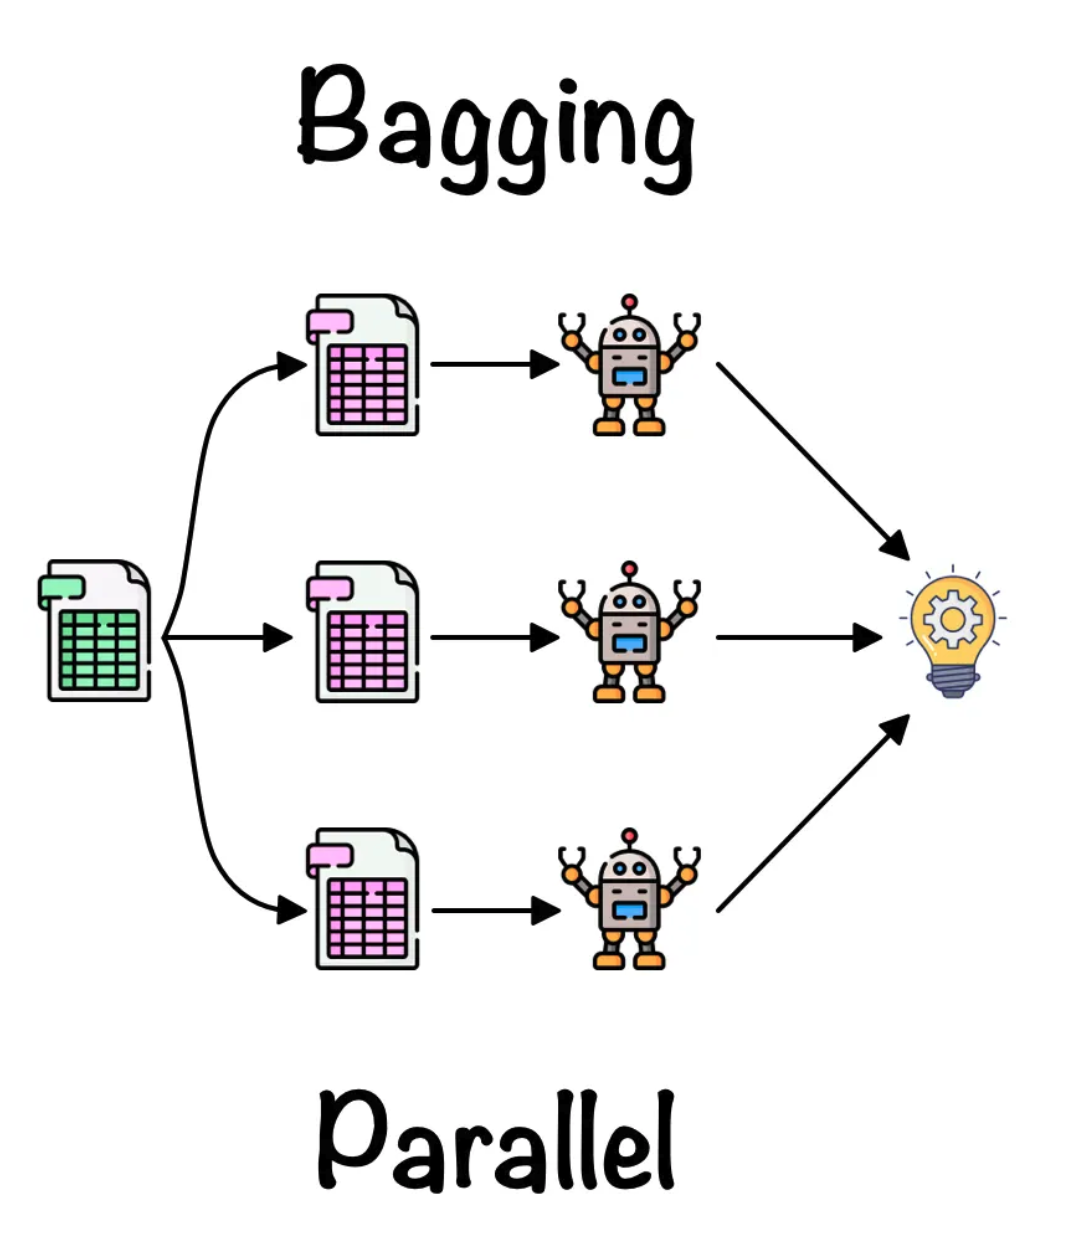
\includegraphics[width=\textwidth]{esb.png}
            \caption{Ensemble Learning[1]}
        \end{figure}
    \end{columns}

    [1] F. López, “Ensemble Learning: Bagging \& Boosting,” Medium, Jan. 18, 2021.


\end{frame}

% Solution
% Partition the training data into several parts, but they do it randomly. I want to do it in a more reasonable way, using co-clustering and make the ensemble process more efficient.

\begin{frame}
    \frametitle{Proposed Solution: Co-clustering for Data Partitioning}
    \begin{block}{Why Co-clustering?}
        \begin{itemize}
            \item NLP Datasets as Matrices: Natural Language Processing datasets can be effectively represented as matrices, making them suitable for co-clustering.
            \item Improved Communication: Grouping related parts of the data together can reduce communication overhead during parallel processing.
            \item Reduced Training Set Size: Co-clustering similar training data can potentially decrease the size of the training set, thus speeding up the training process.
        \end{itemize}
    \end{block}
\end{frame}


\end{document}

